\subsection{Session 4, Exercise 9}

\lineparagraph{Exercise}

Construct pushdown automata for the following languages.

\begin{enumerate}[a)]
\item $L_a = \{a^nb^m | 2n = m \geq{} 1\}$
\item $L_b = \{a^nb^m | 2n \geq{} m \geq{} n \geq{} 1\}$
\end{enumerate}

\lineparagraph{Solution}

a)

The first one is simpler, since we need to check for twice as many $b$'s as $a$'s. We can count the number of $a$'s in the stack with TWO tokens instead of one, so then the number of tokens in the stack must be equal to the number of $b$'s.

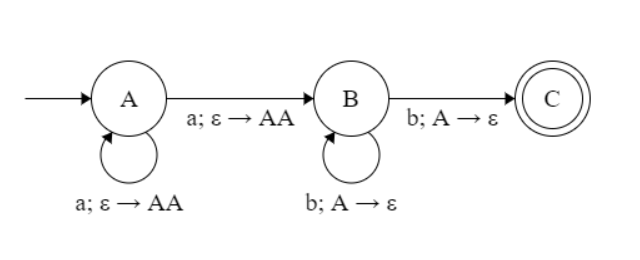
\includegraphics[width=0.5\linewidth]{04/4_9_a.png}

To enforce that the loops run at least once, due to the requirement that $n,m\geq{}1$ ($n\geq{}0.5$ is the same as $n\geq{}1$, since $n$ is an integer), we used non-epsilone transitions between the states, and copied the loop's transition to the existing transitions from the states as well.

TODO Proof

b)

The second one is more complex, since the number of $b$'s is now anywhere between $2n$ and $n$! How do we enforce $2n \geq{} m \geq{} n$? We just did it with $2n = m$, also if it were only $n = m$, we could replace the $a; \varepsilon \rightarrow AA$ transitions with  $a; \varepsilon \rightarrow A$ transitions. But how do we check for in-between these two numbers?

We will rely on non-determinism again:

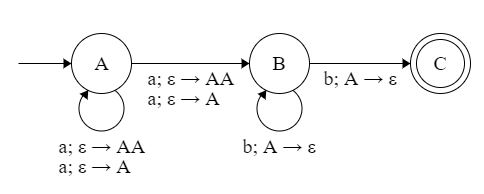
\includegraphics[width=0.5\linewidth]{04/4_9_b.png}

We use both $a; \varepsilon \rightarrow A$ and $a; \varepsilon \rightarrow AA$. The PDA will nondeterministically use either the first or the second transition and push either 1 or 2 $A$'s on the stack. So the number of $A$'s on the stack will be anywhere between $2n$ and $n$, and there will exist a computational branch (if the word is in the language) where their number will be equal to $m$ and the word will be accepted.